\section{Dynamic Systems}

\label{sec:dynamicsystems}

This section covers deterministic and randomized dynamic systems in theory and gives a few intuitive examples of dynamic systems.

Dynamic systems are systems whose development over time can be described by a single or a set of mathematical equations. Although these equations may not always be symbolically solvable they describe the system's dynamics perfectly. Examples include the time-varying temperature of an object as it is placed in the oven or the voltage across an inductor.

\begin{figure}
\begin{center}
\begin{tikzpicture}
\usetikzlibrary{patterns}
\tikzstyle{ground}=[fill,pattern=north east lines,draw=none,minimum width=0.75cm,minimum height=0.3cm]
\node (ground) [ground] at (0,0) {};
\node (angle) at (0.35,-2) {$\phi$};
\draw (0,-0.15) -- (1.4,-4);
\draw[dashed] (0,-0.15) -- (0,-4.5);
\draw[->,>=stealth',semithick] (0.5,-1.5) arc[radius=1.2, start angle=300, end angle=275];
\fill[black] (1.4,-4) circle (.15);
\node (length) at (1.1,-2) {$l$};
\end{tikzpicture}
\end{center}
\caption{1-dimensional mathematical pendulum}
\label{1dpendulum}
\end{figure}

A common example of dynamic systems is the ideal one-dimensional mathematical pendulum seen in Figure~\ref{1dpendulum}. By considering the forces on the pendulum or it's energy it is quite simple to deduce the following differential equation to describe the system \cite{physics}:

\[
0 = \frac{g}{l}\cdot sin(\phi(t))+\ddot{\phi}(t)
\]

With the small-angles assumption

\[
sin(\phi(t))\approx\phi(t)
\]

the solution of the differential equation is

\[
\phi(t) = \hat{\phi} \cdot sin( \sqrt{\frac{g}{l}} \cdot t + {\phi}_0)
\]

where $\hat{\phi}$ is the semi-amplitude and ${\phi}_0$ the phase at time $t=0$. This equation describes the simplified dynamic system perfectly for all times.

An interesting property of the pendulum system is that given the same initial state and excitation (eg. initial angle at $20 ^{\circ}$ and speed $0$), the system will always respond the same way as time progresses. This property is called determinism and guarantees that given the same excitation and initial state the system will always develop identically over time. Systems that posess this property are called \textit{deterministic dynamic systems} and differ greatly from the opposed \textit{randomized dynamic systems}.

\textit{Randomized dynamic systems} are dynamic systems with an element of \textit{randomness}. The consequence of this is that the same initial conditions and excitation do not guarantee an identicial system response. A trivial example of a discrete randomized dynamic system is the following:


\begin{align}
q[n+1] &=\left q[n] + x[n] + e[n]\right \nonumber\\
y[n] &=\left q[n] + x[n]\right \nonumber
\end{align}

where $x[n]$ is the input, $e[n]$ is white noise and $y[n]$ the output at time $n$. If this system is provided with the same input signal twice, the resulting output signal is likely to be slightly different. This is caused by the inherit randomness of a white noise input.

The above example touches on an important point in the field of signal theory and system dynamics. The pendulum example also differs from the white noise example because the former is defined in \textit{continuous time} whilst the latter is defined in \textit{discrete time}. A continuous time system is defined for any time value $t \in T$, where $T$ is the system's time space. A discrete time system is, on the other hand, only defined on a subset of the time line $T$, at discrete times $n \in N \subset T$.

A simple example to illustrate this point is the comparison of the continuous and the discrete sine functions:

\begin{align}
y(t) &=\left sin(t),\right \nonumber \\
y[n] &=\left sin(n) = sin(n \cdot T_s). \right \nonumber
\end{align}

Here $y[n]$ is the discrete-time version of the continuous time system $y(t)$. $y[n]$ is produced by \textit{sampling} $y(n)$ with the sampling frequency $f_s=\frac{1}{T_s}$. This means that whilst $y(t)$ is defined for all times $t$, $y[n]$ is only defined for the times 

\begin{align}
&n \in N \nonumber \\
where& \nonumber \\
N &= n\cdot T_s\ \forall\ (n\ \in\ \mathbb{Z}) \nonumber \\
  &= [-\infty \cdot T_s,-(\infty  -1) \cdot T_s,\cdots,-1 \cdot T_s,0,-1 \cdot T_s,\cdots,(\infty-1) \cdot T_s,\infty \cdot T_s]. \nonumber
\end{align}

\begin{figure}
\begin{center}
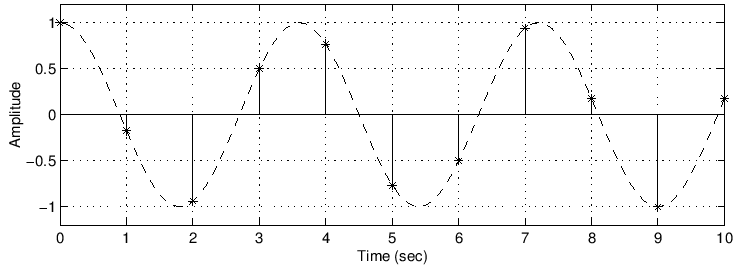
\includegraphics[width=12cm]{media/disc_sine_cont}\\
\end{center}
\caption{Sampling of a continuous sine signal with sampling rate: $\frac{1}{2}$Hz \cite{jos_sine}}
\label{disc_sine_orig}
\end{figure}

\begin{figure}
\begin{center}
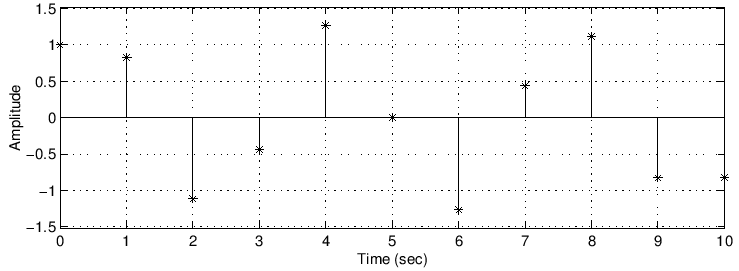
\includegraphics[width=12cm]{media/disc_sine_disc}\\
\end{center}
\caption{Discrete signal produced by sampling a continuous sine signal  with sampling rate: $\frac{1}{2}$Hz \cite{jos_sine}}
\label{disc_sine_disc}
\end{figure}


It is easy to see here that a discrete time system contains less information than a continuous time system. Figure~\ref{disc_sine_orig} shows a sine curve sampled every second (sample points are marked by stars). Figure~\ref{disc_sine_disc} shows the resulting discrete signal. The information density difference between the orignal continuous signal and the sampled discrete signal becomes obvious.  Nonetheless discrete time signals are prevalent because digital systems can only deal with digital (ie. discrete) signals.

The last important property of dynamic systems is the notion of \textit{state}. A system's state is the smallest set of internal and/or external values that represent the entire state of the system. This means that a system's state completely describes that systems condition at a certain time. Coming back to the pendulum example it is clear that the entire system's condition can be described by two variables, the current angle $\phi(t)$ and the current angular velocity $\dot{\phi}(t)$. A definition of these two values at time $t$ completely define the system's condition in past and future times $t\pm (\tau \in \mathbb{R})$. The set of all possible states that a system may find itself in is defined as the \textit{state space} of that system.

\textit{Deterministic dynamic systems} and \textit{randomized dynamic systems} are two extremely useful mathematical constructs and serve as the basis of the more advanced theory of the next few sections.



